

%%%%\section{Mu3e}

The $\mu \rightarrow eee$ decay is a charged lepton flavor violating process strongly suppressed in the Standard Model. New physics mediated either via virtual loop or three diagrams can enhance these rates to values accessible by the next generation of experiments. An interesting feature of this process is 
the possibility to determine the chirality of New Physics, should it be observed with sufficient statistics~\cite{Okada:1999zk}. We present a study to search for $\mu \rightarrow eee$ decay using the FastSim simulation package. The experimental setup, inspired from the Mu3e experiment~\cite{Blondel:2013ia}, is a compact tracker surrounding a target formed by two hollow cones. The tracker consists of 6 layers of cylindrical silicon detectors, each composed of 50 $\mu$m thick silicon sensors mounted on 
50 $\mu$m of kapton. The cones forming the target have a length and radius of 5 cm and 1 cm, respectively. Contrary to Mu3e, we consider an active target made of silicon pixel detectors, 
assuming a pixel size of 50 $\mu$m by 50 $\mu$m. Although not included, a time-of-flight system should be installed as well, providing a time measurement with a resolution between 50 - 500 ps. The apparatus is displayed in Fig.~\ref{Fig::mu3e}, together with a simulated $\mu^+ \rightarrow e^+e^-e^+$ event.

We generate $\mu^+ \rightarrow e^+e^-e^+$ events according to phase space, and reconstruct the decays constraining the tracks to originate from the same position on the target. The vertex 
position is chosen by considering all points from tracks intercepting the target, and choosing the one minimizing the $\chi^2$ of the constrained fit. To further improve the 
resolution, we require the probability of the constrained fit to be greater than 1\%, and a reconstructed muon momentum less than $1 ~\Mev$. The absolute value of the cosine of the polar angle of each electron must also be less than 0.9. The resulting $e^+e^-e^+$ invariant mass distribution, shown in Fig.~\ref{Fig::mu3e}, is fitted with a double-sided Crystal Ball function (a Gaussian with power-law tails on both sides). The Gaussian resolution is found to be 0.3~\Mev\ for a signal efficiency of 27\%. 

To achieve a single event sensitivity at the level of $5\times\sim 10^{-18}$ after a 3-year run, a rate of stopped muons in the target of the order of $8\times 10^{9}$ is needed, assuming 
a reconstruction efficiency of $\sim 27\%$. For the purpose of estimating background contributions, we define a signal window as $ 104.9 < m_{eee} < 106.5 ~\Mev$, containing approximately 90\% of the signal. 

\begin{figure}[htb]
\begin{center}
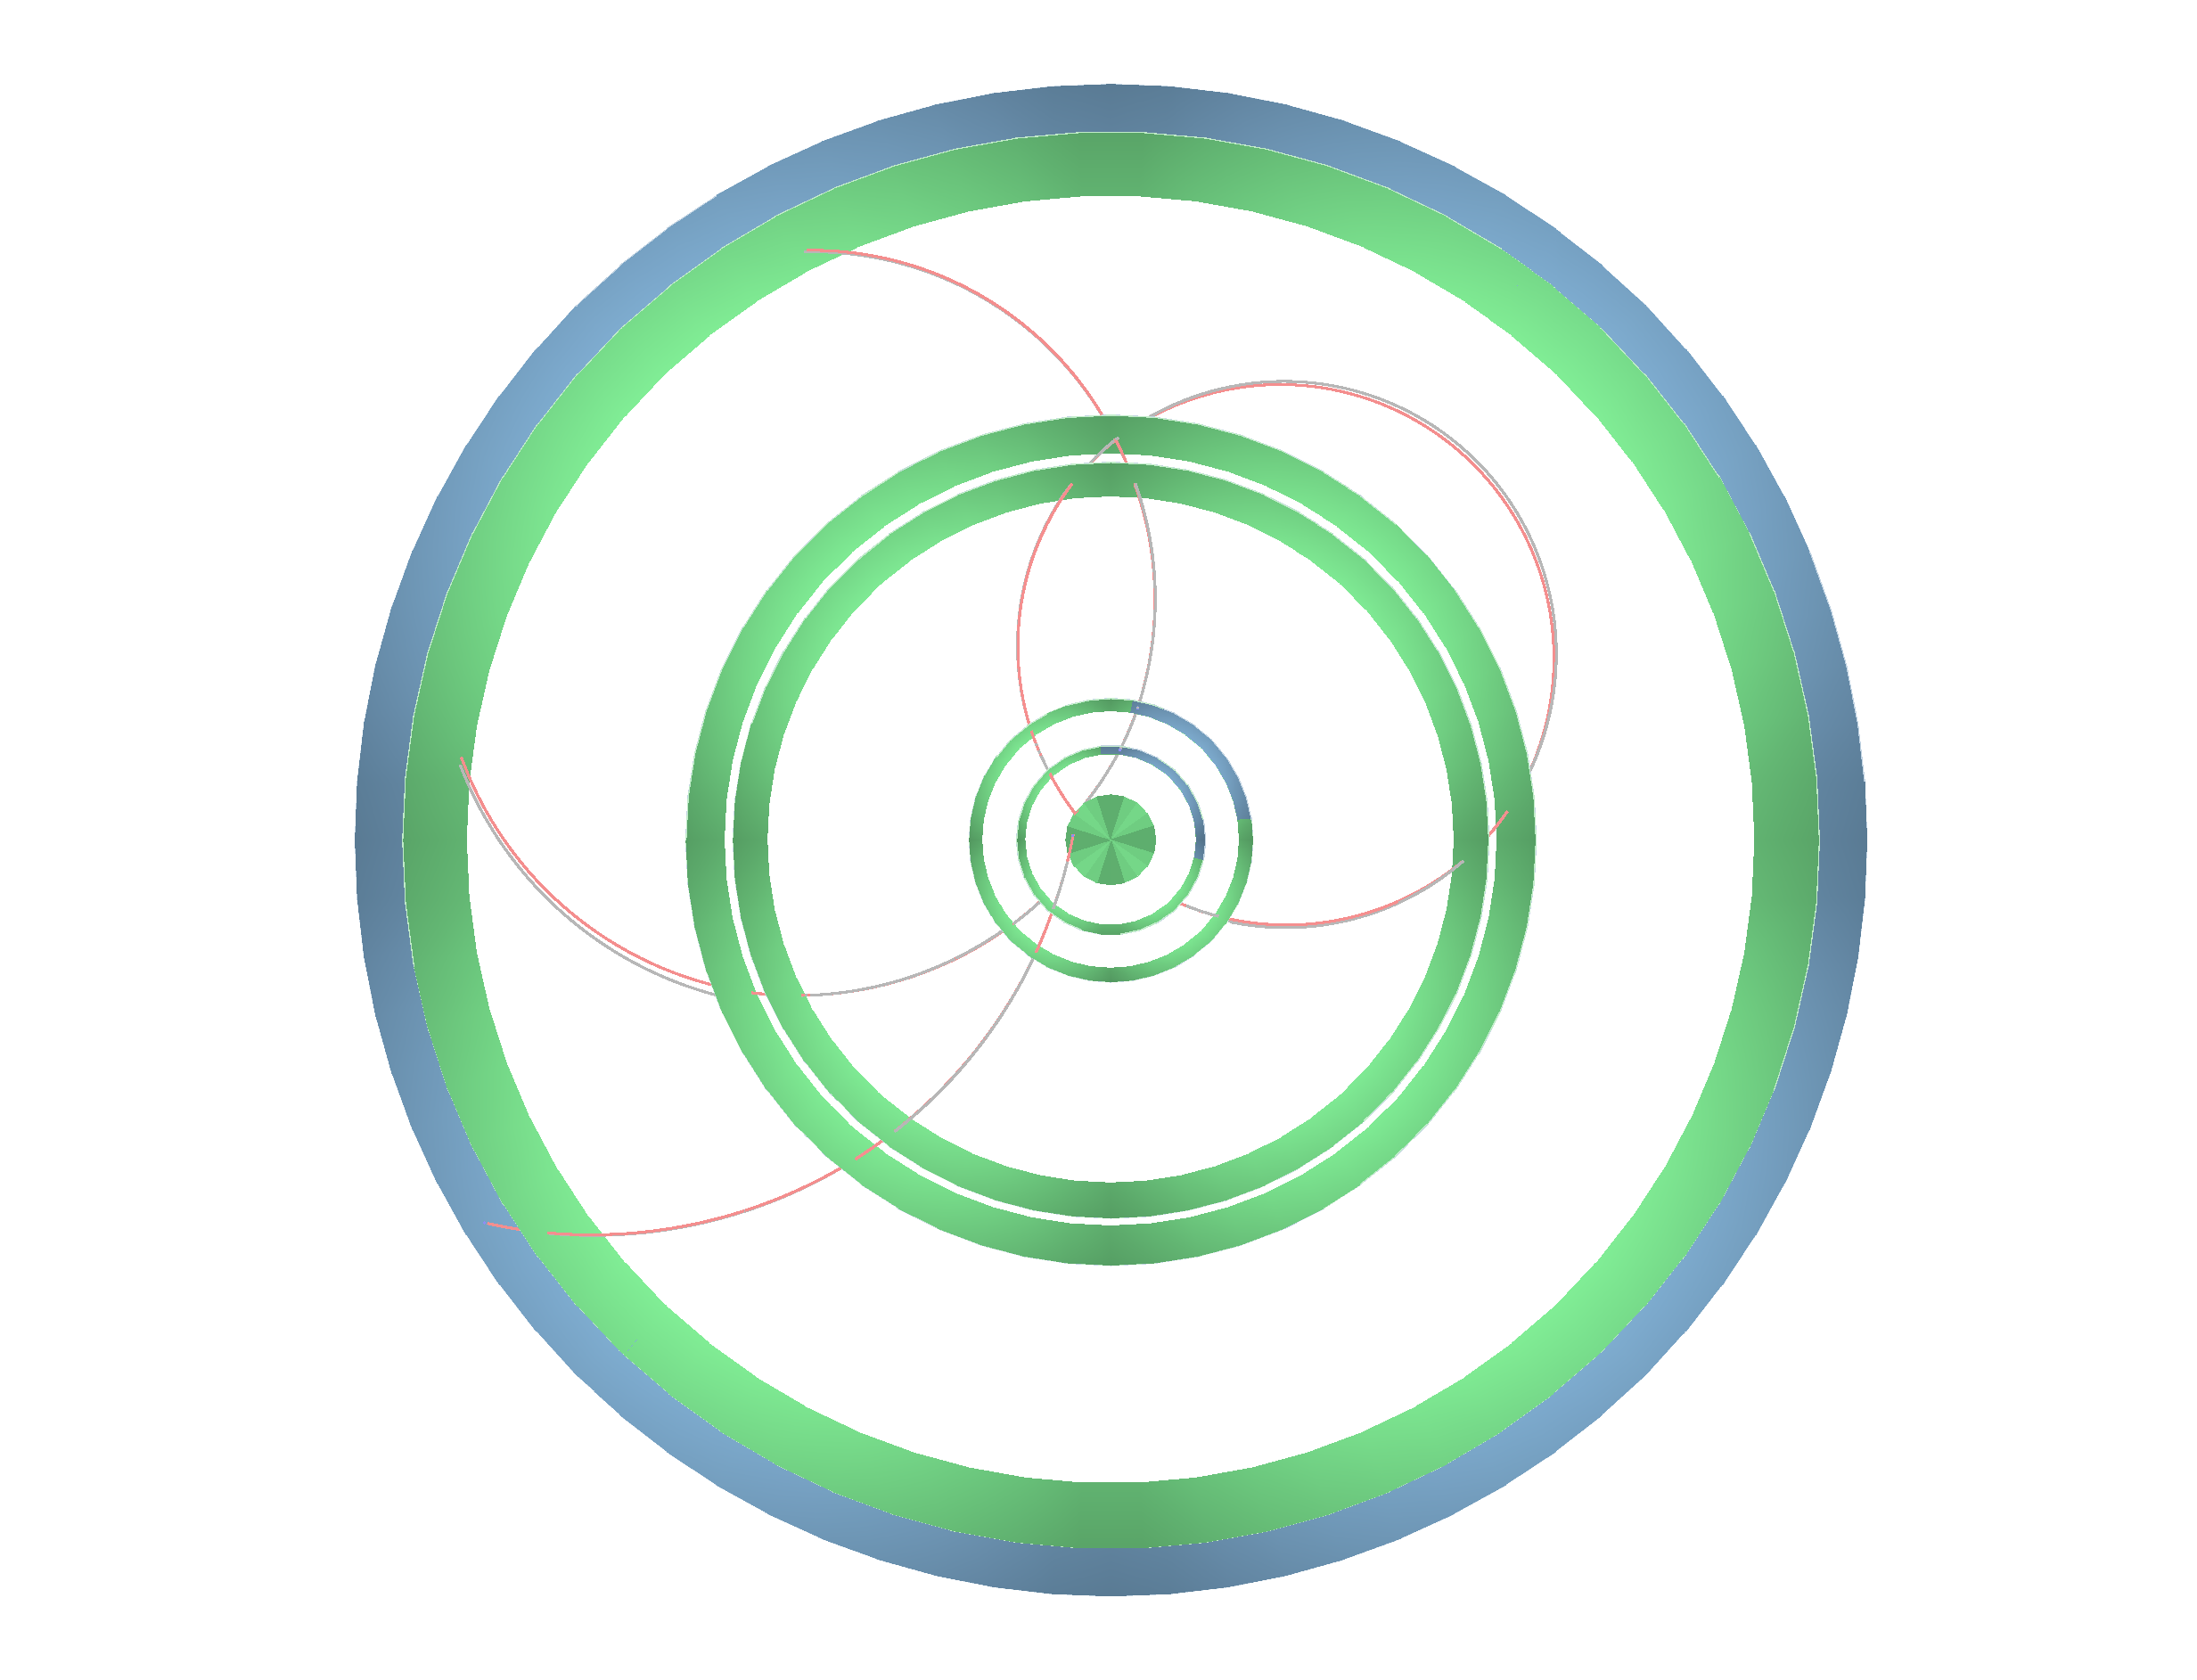
\includegraphics[width=0.45\textwidth]{ChargedLeptons/Figures/event.pdf}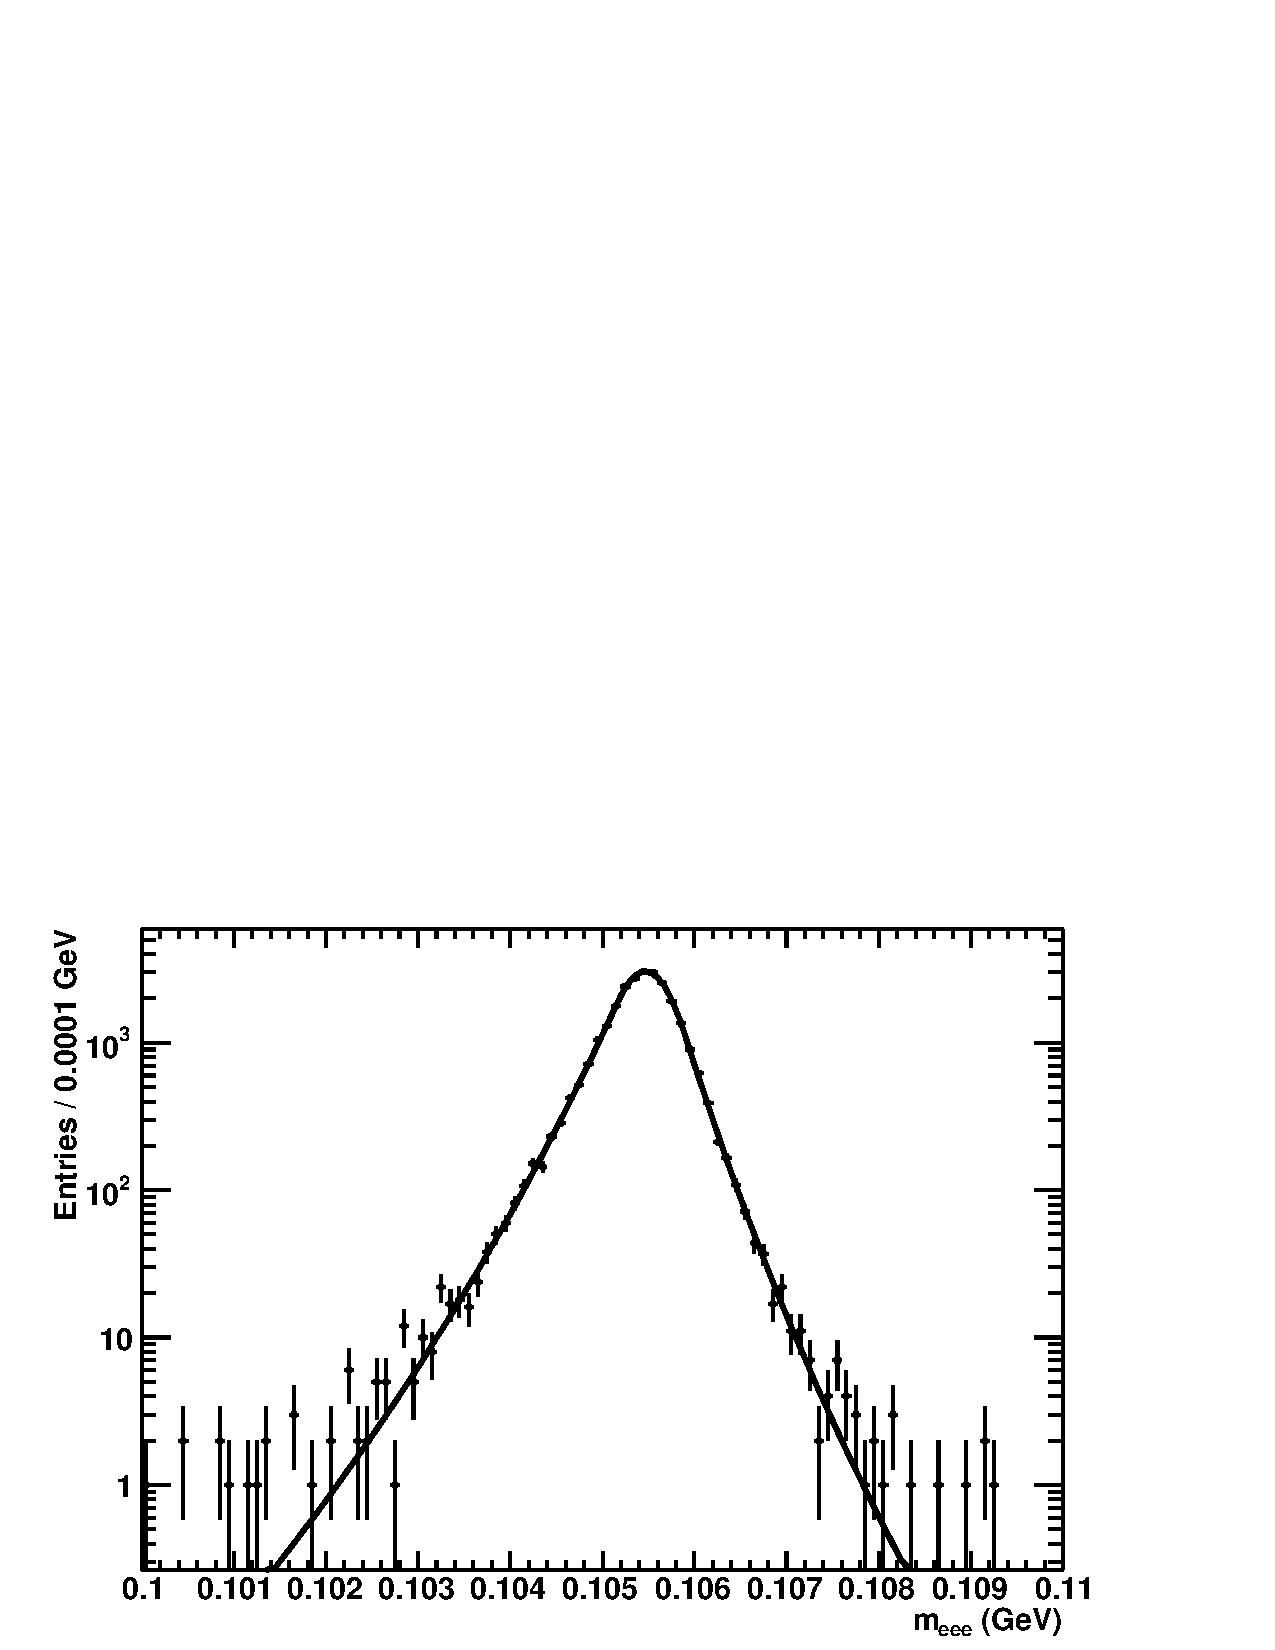
\includegraphics[width=0.45\textwidth]{ChargedLeptons/Figures/resoFit.pdf}
\end{center}
\caption{Left: Display of the experimental setup, together with a simulated $\mu^+ \rightarrow e^+e^-e^+$ event. 
Right:  The $e^+e^-e^+$ invariant mass distribution after all selection criteria are applied fitted by a 
sum of two Gaussian functions.}
\label{Fig::mu3e}
\end{figure}

An important background arises from $\mu \rightarrow e^+e^-e^+ \nu\nu$ events where the two neutrinos carry almost no energy. We estimate its contribution to be about 7.5 events by convolving the branching fraction with the resolution function and integrating in the signal region, using an efficiency of 27\%. One must note that this background depends strongly on the tail resolution, and small improvements translate into large reductions of this contamination. For example, decreasing the thickness of the silicon sensors and the supporting kapton structure by 20\% (40\%) reduces the background to $\sim 4$ ($\sim 1$) events. Additional improvements of the reconstruction algorithms might further ameliorate the resolution and reduce this contamination.

We consider accidental backgrounds produced by the combination of a Michel decay and a radiative Michel decay (2M$\gamma$ decays), or three simultaneous Michel decays (3M decays), where one positron is misreconstructed or produces an electron by interacting within the detector. In both cases, we assume that
the decays occur within the same pixel in the active target and within the same time window, taken to be 250~ps. This yields position and time suppression factors $\delta S = 7.8\times 10^{-7}$ and $\delta t = 2.5\times 10^{-10}$, respectively. The expected number of background events per second is:
%
$$N_{2M\gamma} = {R_\mu}^2 \delta S \delta t {B(\mu^+ \rightarrow e^+ \nu_e \bar\nu_\mu)}^2 B(\mu^+ \rightarrow e^+ \nu_e \bar\nu_\mu \gamma) P(\gamma \rightarrow e^+ e^-)  P_\mu  \simeq 0.33 P_\mu$$
$$N_{3M} = {R_\mu}^3(\delta S)^2 {B(\mu^+ \rightarrow e^+ \nu_e \bar\nu_\mu)}^3 (\delta t)^2 P_\mu \simeq 0.02 P_\mu$$
%
where $P(\gamma \rightarrow e^+ e^-)\sim 0.18\%$ is the probability of photon conversion in the target and $P_\mu$ denotes the probability to reconstruct a muon candidate after all selection criteria are applied. We estimate the factors $P_\mu \sim {\cal O}(10^{-8})$ for 2M$\gamma$ decays and $P_\mu \sim {\cal O}(10^{-9})$ for 3M decays with our simulation. For a 3-year run and with a rate of $8\times 10^{9}$ stopped muons per second, both backgrounds are found to be less than an event.

In summary, we outline the requirements needed to improve by an order of magnitude the projected $\mu \rightarrow eee$ 
sensitivity of the mu3e experiment. We study a similar design, with the addition on an active target instead of a passive one. Assuming a 3-year run, a rate of $8\times 10^{9}$ stopped muons in the target per second would be required. Relatively modest improvements on the resolution are also needed to maintain the irreducible background at an appropriate level, while an active target proves to be essentially in the reduction of accidental 
backgrounds. 







